\section*{Outline and motivation}

In previous lectures we have discussed how travel time and waveform observations can be used to determine variations in
 elastic wave speeds within the Earth. Nothing has, however, been said about \textbf{density}, with this parameter being key to 
 understanding both the Earth's interior composition and dynamics. To learn about density, we need to study the 
 \textbf{long-period free oscillations of the Earth}. This is because \textbf{self-gravitation}, and hence density, plays a vital role in 
 their physics. Within this lecture we will return to basic elastodynamics, and show how gravitational forces can be included 
 into the equations of motion. We also explain how the \textbf{Earth's rotation} enters into the problem. Having obtained the 
 equations of motion, we perform a \textbf{scaling analysis} to determine the relative importance of the different terms, and 
 conclude that at short enough periods the effects of self-gravitation and rotation can be safely neglected, and hence 
 the earlier parts of this course remain valid.

\section*{A review of Newtonian gravitation}

Consider the motion $\bphi$ of an elastic body relative to a reference body $M$, and write $M_{t}$ for 
the instantaneous volume of space occupied at time $t$. At this instant in time, the gravitational potential of the 
body satisfies Poisson's equation
\begin{equation}
\nabla^{2}\phi=4\pi G\varrho,
\label{eq:1}
\end{equation}
in $\mathbb{R}^{3}$, where $G$ is the universal gravitational constant, and $\varrho$ is the spatial density. The gravitational 
acceleration associated with this potential is given by
\begin{equation}
g_{i}=-\frac{\partial\phi}{\partial x_{i}}.
\label{eq:2}
\end{equation}
Poisson's equation is subject to the conditions that $\phi$ tends to zero at infinity, while across any 
jumps in density we have the continuity conditions
\begin{equation}
[\phi]_{-}^{+}=0,\quad [g_{i}\hat{n}_{i}]_{-}^{+}=0,
\label{eq:3}
\end{equation}
where $[\cdot]_{-}^{+}$ denotes the jump in a quantity in the direction of the outward normal.
The closed form solution to this problem is given by
\begin{equation}
\phi(\mathbf{y},t)=-G\int_{M_{t}}\frac{\varrho(\mathbf{y}',t)}{[(y_{i}-y_{i}')(y_{i}-y_{i}')]^{\frac{1}{2}}}\dd^{3}\mathbf{y}',
\label{eq:4}
\end{equation}
and differentiating, we similarly find
\begin{equation}
g_{i}(\mathbf{y},t)=-G\int_{M_{t}}\frac{\varrho(\mathbf{y}',t)(y_{i}-y_{i}')}{[(y_{j}-y_{j}')(y_{j}-y_{j}')]^{\frac{3}{2}}}\dd^{3}\mathbf{y}'.
\label{eq:5}
\end{equation}

For the Earth, the equilibrium gravitational acceleration and the pressure that it produces are shown in Fig.~\ref{fig:1}. These 
were calculated from the radial density profile of the model PREM; where that density comes from is a question we return 
to in Lecture~24, since it is the free oscillations discussed there that provide the main constraint on it. Note that $g$ 
is close to $10\,\mathrm{m\,s^{-2}}$ throughout the mantle, reaching its largest value at the core--mantle boundary, and 
decreases roughly linearly through the core.

\begin{figure}[htbp]
\centering
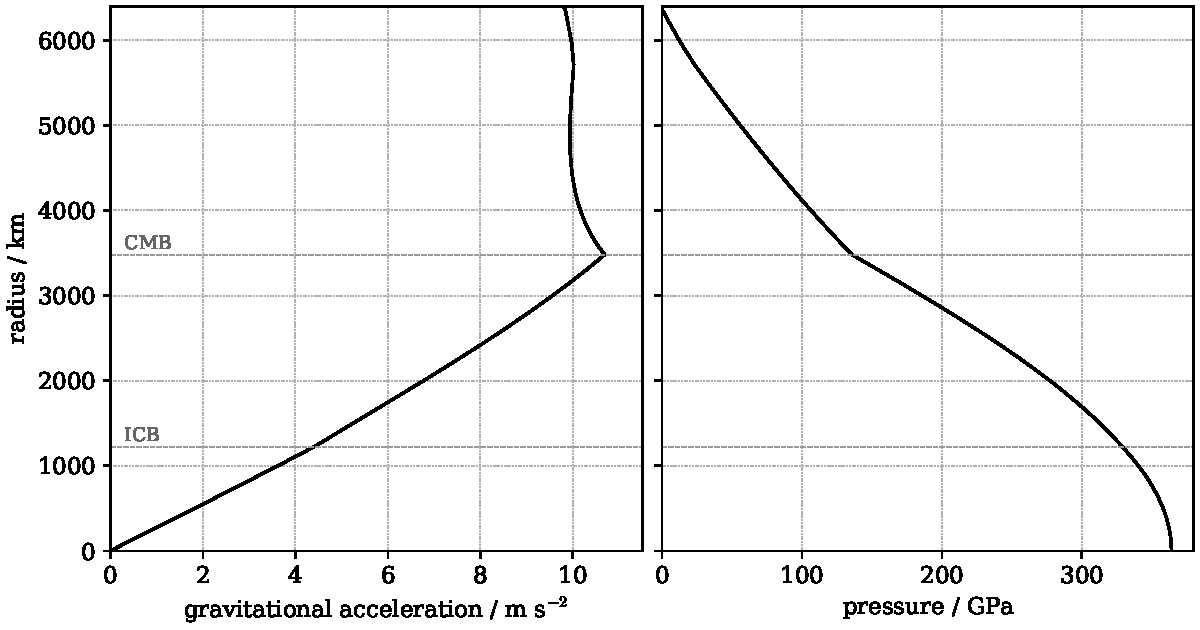
\includegraphics[width=0.85\textwidth]{figures/L9F1.pdf}
\caption{Gravitational acceleration (left) and pressure (right) as functions of radius in the earth model PREM, calculated 
from its density profile. The dashed lines mark the core--mantle boundary (CMB) and inner core boundary (ICB).}
\label{fig:1}
\end{figure}

It will be convenient to define the \textbf{referential gravitational potential} by
\begin{equation}
\zeta(\mathbf{x},t)=\phi[\bphi(\mathbf{x},t),t],
\label{eq:6}
\end{equation}
which is a time-dependent field on the reference body, $M$. We recall from Lecture~13 that the volume elements in 
the reference body and physical space are related by $\dd^{3}\mathbf{y} = J(\mathbf{x},t)\dd^{3}\mathbf{x}$ with $J=\det(\mathbf{F})$ 
the Jacobian of the motion. We can then change variables within eq.~(\ref{eq:4}) and use the definition of $\zeta$ in eq.~(\ref{eq:6}) to obtain
\begin{equation}
\zeta(\mathbf{x},t)=-G\int_{M}\frac{\rho(\mathbf{x}')}{\{[\varphi_{i}(\mathbf{x},t)-\varphi_{i}(\mathbf{x}',t)]
[\varphi_{i}(\mathbf{x},t)-\varphi_{i}(\mathbf{x}',t)]\}^{\frac{1}{2}}}\dd^{3}\mathbf{x}',
\label{eq:7}
\end{equation}
where from Lecture~13 we know that conservation of mass requires
\begin{equation}
\rho(\mathbf{x})=J(\mathbf{x},t)\varrho[\bphi(\mathbf{x},t),t],
\label{eq:8}
\end{equation}
with $\rho$ the \textbf{referential density}. In a similar manner, we define the \textbf{referential gravitational acceleration} by
\begin{equation}
\gamma_{i}(\mathbf{x},t)=g_{i}[\bphi(\mathbf{x},t),t],
\label{eq:9}
\end{equation}
which from eq.~(\ref{eq:5}) can be written
\begin{equation}
\gamma_{i}(\mathbf{x},t)=-G\int_{M}\frac{\rho(\mathbf{x}')[\varphi_{i}(\mathbf{x},t)-\varphi_{i}(\mathbf{x}',t)]}
{\{[\varphi_{j}(\mathbf{x},t)-\varphi_{j}(\mathbf{x}',t)][\varphi_{j}(\mathbf{x},t)-\varphi_{j}(\mathbf{x}',t)]\}^{\frac{3}{2}}}\dd^{3}\mathbf{x}'.
\label{eq:10}
\end{equation}

\subsection*{Gravitational binding energy}

At each instant of time we can associate a \textbf{gravitational binding energy} with the elastic body. This is the energy 
that would be required to assemble the body from matter dispersed at infinity, assuming that its constituent parts 
are acted on only by their mutual gravitational attraction. Because gravity is a conservative force, the binding 
energy is independent of the details of the assembly. 

Suppose that the mass of the body is already in place, 
and that its spatial density and gravitational potential are denoted by $\varrho$ and $\phi$. To determine an 
expression for the binding energy we will consider how this quantity changes due to an infinitesimal addition 
of mass to the body. By definition of the gravitational potential, the work required to bring in an additional 
mass element $\delta\varrho \dd^{3}\mathbf{y}$ from infinity to a point $\mathbf{y}$ within the body is
 $\delta\varrho\,\phi\dd^{3}\mathbf{y}$. 
The change in the binding energy associated with a perturbation $\delta\varrho$ to the body's density is, therefore, given by
\begin{equation}
\delta\mathcal{V}_{g}=\int_{M_{t}}\delta\varrho\,\phi \dd^{3}\mathbf{y},
\label{eq:11}
\end{equation}
to first-order accuracy. Using the perturbed Poisson's equation $\nabla^{2}\delta\phi=4\pi G\delta\varrho$ for 
the resulting change in gravitational potential, we can write this increment to the binding energy as
\begin{equation}
\delta\mathcal{V}_{g}=\frac{1}{4\pi G}\int_{M_{t}}\left(\frac{\partial^{2}\delta\phi}{\partial y_{i}\partial y_{i}}\right)\phi
\dd^{3}\mathbf{y}=\frac{1}{4\pi G}\int_{\mathbb{R}^{3}}\left(\frac{\partial^{2}\delta\phi}{\partial y_{i}\partial y_{i}}\right)\phi\dd^{3}\mathbf{y},
\label{eq:12}
\end{equation}
where the final equality follows from the fact that $\nabla^{2}\delta\phi=0$ outside of the instantaneous 
body $M_{t}$. Using the identity
\begin{equation}
\left(\frac{\partial^{2}\delta\phi}{\partial y_{i}\partial y_{i}}\right)\phi=\frac{\partial}{\partial y_{i}}
\left(\phi\frac{\partial\delta\phi}{\partial y_{i}}\right)-\frac{\partial\phi}{\partial y_{i}}\frac{\partial\delta\phi}{\partial y_{i}},
\label{eq:13}
\end{equation}
and applying the divergence theorem we obtain
\begin{equation}
\delta\mathcal{V}_{g}=-\frac{1}{4\pi G}\int_{\mathbb{R}^{3}}\frac{\partial\phi}{\partial y_{i}}\frac{\partial\delta\phi}{\partial y_{i}}\dd^{3}\mathbf{y},
\label{eq:14}
\end{equation}
where we have used the continuity of the potentials and their normal derivatives across $\partial M_{t}$, while the 
surface integral at infinity vanishes since, at large distances $r$, $\phi$ decays like $r^{-1}$ and $\|\nabla\delta\phi\|$ 
like $r^{-2}$. It follows that the increment to the gravitational binding energy can be written
\begin{equation}
\delta\mathcal{V}_{g}=\delta\left(-\frac{1}{8\pi G}\int_{\mathbb{R}^{3}}\frac{\partial\phi}{\partial y_{i}}
\frac{\partial\phi}{\partial y_{i}}\dd^{3}\mathbf{y}\right),
\label{eq:15}
\end{equation}
and so we arrive at the result
\begin{equation}
\mathcal{V}_{g}=-\frac{1}{8\pi G}\int_{\mathbb{R}^{3}}\frac{\partial\phi}{\partial y_{i}}\frac{\partial\phi}
{\partial y_{i}}\dd^{3}\mathbf{y}.
\label{eq:16}
\end{equation}

Using Poisson's equation for $\phi$, we can write the integrand of the above expression in the form
\begin{equation}
\frac{\partial\phi}{\partial y_{i}}\frac{\partial\phi}{\partial y_{i}}=\frac{\partial}{\partial y_{i}}
\left(\phi\frac{\partial\phi}{\partial y_{i}}\right)-\phi\left(\frac{\partial^{2}\phi}{\partial y_{i}
\partial y_{i}}\right)=\frac{\partial}{\partial y_{i}}\left(\phi\frac{\partial\phi}{\partial y_{i}}\right)-4\pi G\varrho\phi,
\label{eq:17}
\end{equation}
and applying the divergence theorem we obtain
\begin{equation}
\mathcal{V}_{g}(t)=\frac{1}{2}\int_{M_{t}}\varrho(\mathbf{y},t)\phi(\mathbf{y},t)\dd^{3}\mathbf{y},
\label{eq:18}
\end{equation}
where, as above, we have used the continuity of $\phi$ and its normal derivative across $\partial M_{t}$, 
and the surface integral at infinity again vanishes. To include this binding energy into Hamilton's principle, 
it will be necessary to transform eq.~(\ref{eq:18}) to the following integral over the reference body
\begin{equation}
\mathcal{V}_{g}(t)=\frac{1}{2}\int_{M}\rho(\mathbf{x})\zeta(\mathbf{x},t)\dd^{3}\mathbf{x},
\label{eq:19}
\end{equation}
where we have used the definition of the referential gravitational potential in eq.~(\ref{eq:6}) and the statement of 
conservation of mass during the deformation in eq.~(\ref{eq:8}).

\subsection*{The equations of motion relative to inertial space}

Having obtained an appropriate expression for the gravitational binding energy, the equations of motion can 
be readily obtained using Hamilton's principle. The Lagrangian for the problem is
\begin{equation}
\mathcal{L}(\mathbf{x},t,\bphi,\mathbf{v},\mathbf{F})=\frac{1}{2}\rho(\mathbf{x})\|\mathbf{v}\|^{2}
-W(\mathbf{x},t,\mathbf{F})-\frac{1}{2}\rho(\mathbf{x})\zeta(\mathbf{x},t),
\label{eq:20}
\end{equation}
where we note that the elastic strain energy is allowed to be time-dependent to accommodate a seismic source. 
An important point about this Lagrangian is that it is \textbf{non-local} due to the gravitational binding energy. This 
means that the value of the Lagrangian at a point and time cannot be expressed only in terms of the values of 
the various fields and their derivatives at this point. The physical reason for this non-locality is, of course, 
the \textbf{action-at-a-distance property of Newtonian gravitation}. 

The action for the body takes the usual form
\begin{equation}
\mathcal{S}(\bphi)=\int_{0}^{T}\int_{M}\mathcal{L}[\mathbf{x},t,\bphi
(\mathbf{x},t),\mathbf{v}(\mathbf{x},t),\mathbf{F}(\mathbf{x},t)]\dd^{3}\mathbf{x}\dd t,
\label{eq:21}
\end{equation}
and Hamilton's principle requires that this quantity be stationary about the true motion for all 
perturbations with fixed end points. In obtaining the Euler--Lagrange equations, however, we have to account 
for the non-local nature of the Lagrangian. As ever, the mathematical statement of Hamilton's principle is 
the vanishing of the functional derivative of the action
\begin{equation}
\langle D\mathcal{S}(\bphi)|\delta\bphi\rangle=0,
\label{eq:22}
\end{equation}
for all variations, $\delta\bphi$, subject to the usual fixed-endpoint conditions. Here the 
left-hand side is, by definition, just the linear term in the expansion of $\mathcal{S}(\bphi+
\delta\bphi)$ about $\bphi$. Looking at the form of the action, it is clear that this 
linear term takes the form
\begin{equation}
\langle D\mathcal{S}(\bphi)|\delta\bphi\rangle=\int_{0}^{T}\int_{M}
\left(\frac{\delta\mathcal{L}}{\delta\varphi_{i}}\delta\varphi_{i}+\frac{\delta\mathcal{L}}{\delta v_{i}}
\delta v_{i}+\frac{\delta\mathcal{L}}{\delta F_{ij}}\delta F_{ij}\right)\dd^{3}\mathbf{x}\dd t,
\label{eq:23}
\end{equation}
where we have introduced the convenient notation $\frac{\delta\mathcal{L}}{\delta\varphi_{i}}$, 
$\frac{\delta\mathcal{L}}{\delta v_{i}}$ and $\frac{\delta\mathcal{L}}{\delta F_{ij}}$ for the factors 
multiplying the various perturbations. In the case of a local Lagrangian these factors reduce to normal 
partial derivatives, and hence it is only the term $\frac{\delta\mathcal{L}}{\delta\varphi_{i}}$ that requires 
additional thought. Applying the usual integration by parts steps, we arrive at the Euler--Lagrange equation
\begin{equation}
\frac{\delta\mathcal{L}}{\delta\varphi_{i}}-\frac{\partial}{\partial t}\left(\frac{\delta\mathcal{L}}
{\delta v_{i}}\right)-\frac{\partial}{\partial x_{j}}\left(\frac{\delta\mathcal{L}}{\delta F_{ij}}\right)=0,
\label{eq:24}
\end{equation}
along with the natural boundary condition
\begin{equation}
\frac{\delta\mathcal{L}}{\delta F_{ij}}\hat{n}_{j}=0
\label{eq:25}
\end{equation}
on $\partial M$. 

As in the non-gravitating case we have
\begin{equation}
\frac{\delta\mathcal{L}}{\delta v_{i}}=\rho v_{i},\quad \frac{\delta\mathcal{L}}{\delta F_{ij}}=-\frac{\partial W}{\partial F_{ij}},
\label{eq:26}
\end{equation}
while in the second problem set you will show that
\begin{equation}
\frac{\delta\mathcal{L}}{\delta\varphi_{i}}=\rho\gamma_{i},
\label{eq:27}
\end{equation}
with $\gamma_{i}$ the referential gravitational acceleration as defined above. The equations of motion, therefore, take the expected form
\begin{equation}
\rho\frac{\partial v_{i}}{\partial t}-\frac{\partial T_{ij}}{\partial x_{j}}-\rho\gamma_{i}=0,
\label{eq:28}
\end{equation}
with $T_{ij}=\frac{\partial W}{\partial F_{ij}}$ the first Piola--Kirchhoff stress tensor. The form 
of these equations is not, of course, unexpected. To the balance of linear momentum obtained previously, 
we have simply added the gravitational force acting on the body due to its own mass.

\subsection*{Use of a co-rotating reference frame}
We have obtained the equations of motion for a self-gravitating body with respect to an \textbf{inertial reference} 
frame defined by the ``fixed stars'', and these results could be applied directly to the Earth. As, however, 
the Earth undergoes a nearly steady rotation about its polar axis, it is useful to reformulate the equations 
of motion with respect to a \textbf{non-inertial frame that rotates with the Earth}.

To do this we express the motion as
\begin{equation}
\varphi_{i}(\mathbf{x},t)=\Phi_{i}(t)+R_{ij}(t)\overline{\varphi}_{j}(\mathbf{x},t),
\label{eq:29}
\end{equation}
where $\mathbf{R}(t)$ is a rotation matrix. Here $\bm{\Phi}(t)$ denotes the translation of the reference frame relative 
to inertial space, and $\mathbf{R}(t)$ changes of orientation. The term $\overline{\bphi}(\mathbf{x},t)$ 
 describes the motion relative to the non-inertial frame, and will be called the \textbf{relative motion}.
 
 Differentiating eq.~(\ref{eq:29}) with respect to time 
we see that the velocity relative to inertial space can be written
\begin{equation}
v_{i}=\frac{\ddns \Phi_{i}}{\ddns t}+R_{ij}\left(\frac{\partial\overline{\varphi}_{j}}{\partial t}+R_{kj}\frac{\ddns R_{kl}}{\ddns t}\overline{\varphi}_{l}\right),
\label{eq:30}
\end{equation}
where we have used the identity $R_{ij}R_{kj}=\delta_{ik}$ for rotation matrices. If we differentiate the
companion identity $R_{kj}R_{kl}=\delta_{jl}$ we find
\begin{equation}
\frac{\ddns R_{kj}}{\ddns t}R_{kl}+R_{kj}\frac{\ddns R_{kl}}{\ddns t}=0,
\label{eq:31}
\end{equation}
and hence conclude that $R_{kj}\frac{\ddns R_{kl}}{\ddns t}$ is an \textbf{anti-symmetric matrix}. It follows that we can use the 
alternating tensor to write
\begin{equation}
R_{kj}\frac{\ddns R_{kl}}{\ddns t}=\epsilon_{jml}\Omega_{m},
\label{eq:32}
\end{equation}
for a uniquely determined vector $\bm{\Omega}$. Using this result, the velocity becomes
\begin{equation}
v_{i}=\frac{\ddns \Phi_{i}}{\ddns t}+R_{ij}(\overline{v}_{j}+\epsilon_{jkl}\Omega_{k}\overline{\varphi}_{l}).
\label{eq:33}
\end{equation}
Here $\overline{\mathbf{v}}$ is the velocity as seen from the non-inertial frame, while $\bm{\Omega}$ is the 
\textbf{angular velocity of the frame}. Differentiating again and applying the same ideas, the acceleration relative 
to inertial space can be written
\begin{equation}
\frac{\partial v_{i}}{\partial t}=\frac{\ddns ^{2}\Phi_{i}}{\ddns t^{2}}+R_{ij}\left(\frac{\partial\overline{v}_{j}}{\partial t}+2\epsilon_{jkl}\Omega_{k}\overline{v}_{l}+\epsilon_{jkl}\frac{\ddns \Omega_{k}}{\ddns t}\overline{\varphi}_{l}+\epsilon_{jkl}\epsilon_{lmn}\Omega_{k}\Omega_{m}\overline{\varphi}_{n}\right).
\label{eq:34}
\end{equation}
On the right-hand side we can identify various terms. The first is the acceleration of the frame relative to 
inertial space. Within the brackets we then see, relative to the non-inertial frame, accelerations associated 
with the motion along with the expected \textbf{Coriolis}, \textbf{Euler}, and \textbf{centrifugal} contributions.

We have not yet specified \emph{how} the non-inertial frame is to be chosen. Within seismology the most common 
approach is to take
\begin{equation}
\frac{\ddns \bm{\Phi}}{\ddns t}=\mathbf{0},\quad \frac{\ddns \bm{\Omega}}{\ddns t}=\mathbf{0},
\label{eq:35}
\end{equation}
which corresponds to a frame whose \textbf{origin is static} relative to the ``fixed stars'' but \textbf{rotates steadily}, 
with the angular velocity chosen so that the frame \textbf{approximately co-rotates with the Earth}. The advantage of this 
choice is its simplicity. But it does mean that orbital, rotational, and relative motion of the Earth are mixed 
up within the term $\overline{\bphi}$. A preferable approach is to use the so-called 
\textbf{Tisserand frame} which is defined such that the relative motion, $\overline{\bphi}$, carries no net linear
 or angular momentum.\footnote{See Maitra \& Al-Attar (2024) for details.}
But we will stick to the simpler and more common choice in this course. 

To complete the derivation of the equations of motion in the non-inertial frame, we note from eq.~(\ref{eq:29}) that
\begin{equation}
F_{ij}=R_{ik}\overline{F}_{kj},
\label{eq:36}
\end{equation}
with $\overline{\mathbf{F}}$ the deformation gradient associated with relative motion. Due to material frame 
indifference, we then have $W(\mathbf{x},t,\mathbf{F})=W(\mathbf{x},t,\overline{\mathbf{F}})$ as should be physically  
expected. Using the chain rule, we find
\begin{equation}
\overline{T}_{ij}=\frac{\partial W}{\partial\overline{F}_{ij}}(\overline{\mathbf{F}})=\frac{\partial}{\partial
\overline{F}_{ij}}W(\mathbf{R}\overline{\mathbf{F}})=\frac{\partial W}{\partial F_{kl}}(\mathbf{R}\overline{\mathbf{F}})
\frac{\partial}{\partial\overline{F}_{ij}}(R_{km}\overline{F}_{ml})=R_{ki}T_{kj},
\label{eq:37}
\end{equation}
with the left-hand side the stress associated with $\overline{\bphi}$. Passing the rotation matrix to the 
other side, we have then obtained the useful identity
\begin{equation}
T_{ij}=R_{ik}\overline{T}_{kj},
\label{eq:38}
\end{equation}
between the first Piola--Kirchhoff stress relative to the inertial and non-inertial reference frames. Finally, we put 
eq.~(\ref{eq:29}) into eq.~(\ref{eq:10}) to find the relationship
\begin{equation}
\gamma_{i}=R_{ij}\overline{\gamma}_{j},
\label{eq:39}
\end{equation}
between the referential gravitational acceleration in the two frames, with $\overline{\bm{\gamma}}$ defined 
exactly as in eq.~(\ref{eq:10}) but with $\overline{\bphi}$ replacing $\bphi$. Using these various 
results we have shown that the equations of motion are equivalent to
\begin{equation}
\rho\left(\frac{\partial\overline{v}_{i}}{\partial t}+2\epsilon_{ijk}\Omega_{j}\overline{v}_{k}+\epsilon_{ijk}
\epsilon_{klm}\Omega_{j}\Omega_{l}\overline{\varphi}_{m}\right)-\frac{\partial\overline{T}_{ij}}{\partial x_{j}}-\rho\overline{\gamma}_{i}=0.
\label{eq:40}
\end{equation}
These equations are identical in form to those in an inertial frame except for the inclusion of the Coriolis and 
centrifugal accelerations -- the Euler acceleration has been removed because we have restricted attention to a 
steadily rotating frame. From this point on we will consistently work in the approximately co-rotating frame, 
and hence will simplify notation by dropping overlines on terms linked to the relative motion. 

\subsection*{Linearised equations of motion}

As ever, our main concern is with the linearised equations of motion about an equilibrium state.
Strictly, we should use the term \textbf{relative equilibrium}, as the body is now 
undergoing a steady rotation relative to inertial space. We consider a disturbance to the body
caused by a stress glut, and hence take the strain energy to be
\begin{equation}
W(\mathbf{x},t,\mathbf{F})=U(\mathbf{x},\mathbf{C})-s\frac{1}{2}\overline{S}_{ij}(\mathbf{x},t)C_{ij},
\label{eq:41}
\end{equation}
with $s$ a perturbation parameter, and $\overline{\mathbf{S}}$ a given stress glut. As in Lecture~15, the elastic tensor 
that appears below is the second derivative of the time-independent part $U(\mathbf{x},\mathbf{C})$ of this strain energy function. 
In a now standard manner we can 
obtain linearised equations of motion for the displacement vector defined as the first-order term in the expansion
\begin{equation}
\varphi_{i}(\mathbf{x},t)=x_{i}+s\,u_{i}(\mathbf{x},t)+O(s^{2}).
\label{eq:42}
\end{equation}
At zeroth order, the equations of motion take the form
\begin{equation}
\rho\epsilon_{ijk}\epsilon_{klm}\Omega_{j}\Omega_{l}x_{m}-\frac{\partial T_{ij}^{0}}{\partial x_{j}}-\rho\gamma_{i}^{0}=0,
\label{eq:43}
\end{equation}
where $T_{ij}^{0}$ and $\gamma_{i}^{0}$ denote the equilibrium values of the stress tensor and gravitational acceleration. 
We will have more to say about these equations in the following lecture, but for the moment note that there 
must be a balance between the centrifugal and gravitational forces on the body and the resulting equilibrium stress; the 
simplifying assumption of a stress-free equilibrium is no longer an option. 

From the first-order term in the expansion we arrive at the linearised equations of motion for the displacement field
\begin{equation}
\rho\left(\frac{\partial^{2}u_{i}}{\partial t^{2}}+2\epsilon_{ijk}\Omega_{j}\frac{\partial u_{k}}{\partial t}+
\epsilon_{ijk}\epsilon_{klm}\Omega_{j}\Omega_{l}u_{m}\right)-\frac{\partial}{\partial x_{j}}\left(A_{ijkl}
\frac{\partial u_{k}}{\partial x_{l}}\right)-\rho\gamma_{i}^{1}=-\frac{\partial\overline{S}_{ij}}{\partial x_{j}},
\label{eq:44}
\end{equation}
where $\gamma_{i}^{1}$ denotes the first-order perturbation to the referential gravitational acceleration. 
Using a binomial expansion, this term can be written explicitly as
\begin{equation}
\gamma_{i}^{1}=-G\int_{M}\rho'\left(\frac{\delta_{ij}}{[(x_{k}-x_{k}')(x_{k}-x_{k}')]^{3/2}}-
\frac{3(x_{i}-x_{i}')(x_{j}-x_{j}')}{[(x_{k}-x_{k}')(x_{k}-x_{k}')]^{5/2}}\right)(u_{j}-u_{j}')\dd^{3}\mathbf{x}',
\label{eq:45}
\end{equation}
where it is understood that primed terms are functions of the integration variable. The boundary conditions 
for the problem take the expected form
\begin{equation}
A_{ijkl}\frac{\partial u_{k}}{\partial x_{l}}\hat{n}_{j}=\overline{S}_{ij}\hat{n}_{j}.
\label{eq:46}
\end{equation}
The key point is that the inclusion of gravitation and rotation into the problem only requires some additional 
terms in the equations of motion considered so far. It is notable, however, that these are no longer partial 
differential equations, but \textbf{integro-differential equations}, with 
both derivatives and integrals of the unknown functions occurring within the equations of motion. 
Again, this feature derives from the action-at-a-distance property of Newtonian gravitation.

\subsection*{The neglect of self-gravitation and rotation}

We have obtained the linearised equations of motion within a steadily rotating and self-gravitating body. 
It is natural to ask if and why it has been reasonable to neglect these physical phenomena up till this point. 
To do so, we will perform a scaling analysis of the equations. 

We assume that the displacement vector field is 
characterised by a typical amplitude $\|\mathbf{u}\|\sim U$, a length scale $L$ and a time scale $T$. The following 
order-of-magnitude scaling estimates are then immediate
\begin{align}
\rho\frac{\partial^{2}u_{i}}{\partial t^{2}}&\sim\frac{\overline{\rho}U}{T^{2}}, \label{eq:47} \\
\rho\epsilon_{ijk}\Omega_{j}\frac{\partial u_{k}}{\partial t}&\sim\frac{\overline{\rho}\Omega U}{T}, \label{eq:48} \\
\rho\epsilon_{ijk}\epsilon_{klm}\Omega_{j}\Omega_{l}u_{m}&\sim\overline{\rho}\Omega^{2}U, \label{eq:49} \\
\frac{\partial}{\partial x_{j}}\left(A_{ijkl}\frac{\partial u_{k}}{\partial x_{l}}\right)&\sim\frac{\overline{\mu}U}{L^{2}}, \label{eq:50}
\end{align}
where $\overline{\rho}$ and $\overline{\mu}$ denote typical values of density and elastic moduli within the body, 
while $\Omega$ is the magnitude of the rotation vector. The scaling estimate for the gravitational term within 
the equations of motion requires more thought. The referential gravitational potential at equilibrium is given by
\begin{equation}
\zeta_{0}=-G\int_{M}\frac{\rho'}{[(x_{k}-x_{k}')(x_{k}-x_{k}')]^{1/2}}\dd^{3}\mathbf{x}'.
\label{eq:51}
\end{equation}
Taking the gradient of this expression twice, we obtain
\begin{equation}
\frac{\partial^{2}\zeta_{0}}{\partial x_{i}\partial x_{j}}=G\int_{M}\rho'\left(\frac{\delta_{ij}}{[(x_{k}-x_{k}')
(x_{k}-x_{k}')]^{3/2}}-\frac{3(x_{i}-x_{i}')(x_{j}-x_{j}')}{[(x_{k}-x_{k}')(x_{k}-x_{k}')]^{5/2}}\right)\dd^{3}\mathbf{x}',
\label{eq:52}
\end{equation}
Comparing eqs.~(\ref{eq:45}) and (\ref{eq:52}), the contribution of $u_{j}$ to $\gamma_{i}^{1}$ is
$-u_{j}\,\partial^{2}\zeta_{0}/\partial x_{i}\partial x_{j}$, whose magnitude is set by the trace $\nabla^{2}\zeta_{0}=4\pi G\rho$
given by Poisson's equation, and hence we arrive at the desired scaling estimate
\begin{equation}
\rho\gamma_{i}^{1}\sim4\pi G\overline{\rho}^{2}U.
\label{eq:53}
\end{equation}

Using these results, we can quantify the relative importance of the terms within the force balance. First we have
\begin{equation}
\frac{\text{gravitational forces}}{\text{elastic forces}}=\frac{4\pi G\overline{\rho}^{2}U}
{\frac{\overline{\mu} U}{L^{2}}}=\frac{4\pi G\overline{\rho}L^{2}}{\overline{v}^{2}},
\label{eq:54}
\end{equation}
where $\overline{v}=\sqrt{\overline{\mu}/\overline{\rho}}$ represents a typical elastic wave speed in the model. 
This ratio scales like $L^{2}$ where $L$ is the characteristic length scale of the deformation. We conclude that 
for deformations occurring over sufficiently small length scales, gravitational forces will be negligible relative 
to elastic ones. We should then ask whether gravitational forces will ever be of importance within the Earth. To 
answer this, we note that the largest-scale deformation within the Earth can have $L$ equal to its average radius $6371\,\mathrm{km}$.
Recalling that $G=6.67\times10^{-11}\,\mathrm{m^{3}\,kg^{-1}\,s^{-2}}$, and taking as typical values $\overline{\rho}=5000\,
\mathrm{kg\,m^{-3}}$ and $\overline{v}=8000\,\mathrm{m\,s^{-1}}$, we find
\begin{equation}
\frac{\text{gravitational forces}}{\text{elastic forces}}\sim3.
\label{eq:55}
\end{equation}
For such planetary-scale deformations, it follows that gravitational forces are of the same order of magnitude as elastic forces, 
and so cannot be neglected within the dynamics. 

Next, we consider the ratio of the Coriolis and inertial terms, and find
\begin{equation}
\frac{\text{Coriolis term}}{\text{inertial term}}=\frac{\frac{\overline{\rho}\Omega U}{T}}{\frac{\overline{\rho}U}{T^{2}}}=\Omega T.
\label{eq:56}
\end{equation}
It follows that the Coriolis terms will be negligible for motions whose time scale is short relative to the rotation period 
of the Earth. A similar conclusion is readily shown to hold for the centrifugal term. It is known that seismic deformation 
is limited to periods shorter than about one hour, and so rotational effects play a relatively small (but not negligible) 
role in the problem. There are, however, processes at longer periods, e.g.\ those associated with solid-Earth tides, for which 
rotation becomes very important.

The conclusions of this scaling analysis can be checked directly by computing synthetic seismograms in a spherically
symmetric earth model with gravitation and with all gravitational effects switched off, i.e.\ with neither the equilibrium
gravitational field nor its perturbation included in the equations of motion, as shown in Fig.~\ref{fig:2}, where attenuation has been  
neglected so that the long-period waves persist over the six hours shown.\footnote{The calculations use the 
program \texttt{yspec}, which solves the equations of motion of this lecture in a spherically symmetric earth model by direct 
numerical integration in the frequency domain (Al-Attar \& Woodhouse 2008).} Over the full frequency band of the 
calculation, which extends to $50\,\mathrm{mHz}$, the two seismograms are indistinguishable for the first few hours, and 
they remain so when band-pass filtered to periods shorter than a few minutes, in keeping with the estimate that 
gravitational forces are negligible for deformations on length scales much smaller than the radius of the Earth. 
As the pass band is moved to longer periods, however, differences appear and steadily grow, and in the lowest band, 
at periods between eight and seventeen minutes, they are substantial: the oscillations are slightly but systematically 
slower without gravitation, so that the two waveforms drift apart as the long-period surface waves circle the Earth. 
Even at the shortest periods small differences eventually become visible in the surface waves that have circled the 
Earth several times, since a fractional change in wave speed of only $10^{-4}$ accumulates into a noticeable phase 
shift over the hundreds of cycles they have then completed. These are precisely the deformations whose length scale is comparable 
to that of the planet, and we shall see in Lecture~23 that the periods of the corresponding free oscillations of the Earth are 
altered by self-gravitation.

\begin{figure}[htbp]
\centering
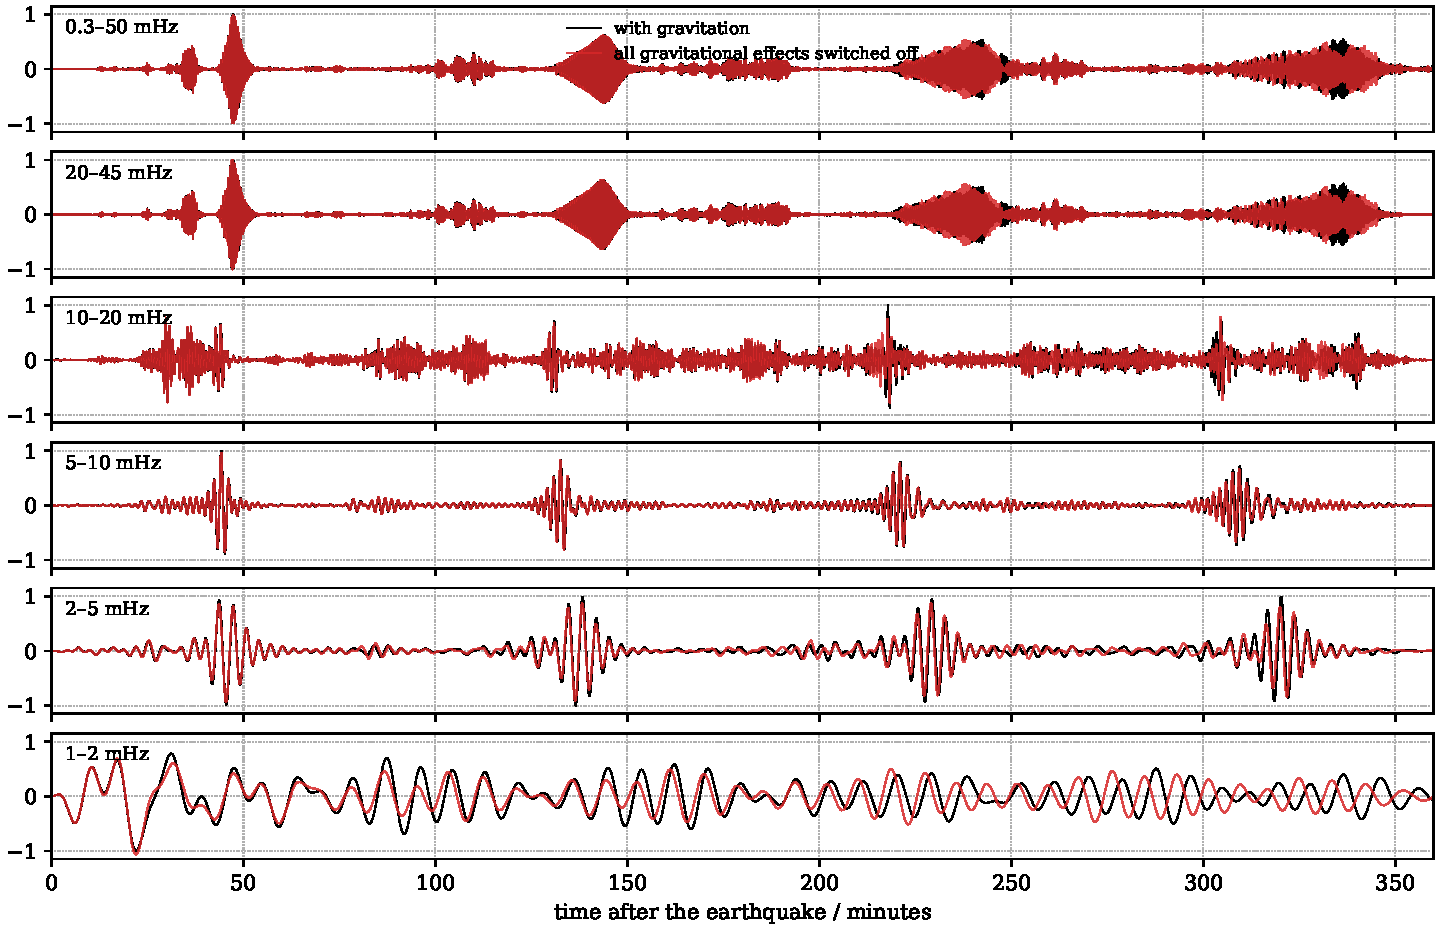
\includegraphics[width=0.95\textwidth]{figures/L9F2.pdf}
\caption{Synthetic vertical-component acceleration seismograms in the earth model PREM for an earthquake of moment magnitude 8 at 
$20\,\mathrm{km}$ depth, recorded at an epicentral angle of $90^{\circ}$, computed with gravitation (black) and with all
gravitational effects switched off (red), i.e.\ with neither the equilibrium gravitational field nor its perturbation.
The top trace shows the full band of the calculation, from $0.3$ to $50\,\mathrm{mHz}$, and those below
it the same seismogram band-pass filtered in successively lower frequency bands. In each panel both traces are normalised
by the maximum of the gravitating one. The  
calculations neglect attenuation, so that the surface waves continue to circle the Earth undiminished over the six hours 
shown. The two calculations differ appreciably only in the lowest bands, and there the differences grow with time as the  
long-period surface waves circle the Earth.}
\label{fig:2}
\end{figure}

\section*{What you need to know and be able to do}
\begin{enumerate}
    \item[(i)] Understand the relevant parts of Newtonian gravity, including the manner in which the gravitational potential 
    and acceleration can be transformed into quantities defined on the reference body.
    \item[(ii)] Know physically what the gravitational binding energy of a planet represents, and how it can be determined.
    \item[(iii)] Know how the gravitational binding energy is incorporated into the Lagrangian, and how the equations of 
    motion can be obtained. The full derivation is too long to be examined, but you may be asked to reproduce parts of it 
    given appropriate information and guidance.
    \item[(iv)] Perform scaling arguments to determine the relative size of terms within an equation, and to determine 
    whether some of them might be negligible. This is a technique required throughout this course, and you should ensure you are happy with it.
\end{enumerate}
